\chapter{Multipath Propagation \& Fading (Rayleigh \& Rician)}
\label{ch:multipath}

\begin{nontechnical}
\textbf{Multipath is like hearing echoes in a canyon}---radio signals bounce off buildings/walls and arrive at your phone from multiple directions at slightly different times.

\textbf{The problem:}
\begin{enumerate}
\item Signal travels \textbf{direct path} from tower to phone (fast)
\item Same signal bounces off buildings (slower paths)
\item All copies arrive at different times and \textbf{interfere} with each other
\item Sometimes they add up (strong signal), sometimes they cancel out (weak signal)
\item This causes \textbf{fading}: signal strength fluctuates wildly as you move!
\end{enumerate}

\textbf{Real-world experience:}
\begin{itemize}
\item \textbf{Driving through city}: Cell signal goes from 5 bars to 2 bars back to 5 bars---that's multipath fading
\item \textbf{WiFi dead spots}: Walk 1 meter and signal drops---destructive interference from multipath
\item \textbf{Crackling old TV}: Picture would fade in/out---multipath from distant transmitter
\end{itemize}

\textbf{Two types:}
\begin{itemize}
\item \textbf{Rayleigh fading} (no direct path): All paths bounced/scattered, signal varies randomly (can drop 30+ dB!), common in dense urban areas
\item \textbf{Rician fading} (strong direct path + echoes): One dominant LOS path + weaker echoes, less severe fading, common in suburban areas
\end{itemize}

\textbf{How engineers fix it:} MIMO (multiple antennas sample different fade patterns), OFDM (spread data across many frequencies---some fade, others don't), Adaptive coding (slow down when fading is bad), Interleaving (spread bits over time so fades don't wipe out whole packets).

\textbf{Fun fact:} Multipath is why 5G uses higher frequencies---shorter waves = less bouncing = more predictable (but shorter range!).
\end{nontechnical}

\section{Overview}

\textbf{Multipath propagation} occurs when RF signals reach the receiver via \textbf{multiple paths} simultaneously, each with different delay, amplitude, and phase characteristics.

\begin{keyconcept}
In mobile and urban environments, multipath fading is the \textbf{dominant impairment}---often more severe than thermal noise. Rayleigh fading can degrade BER by 1000× compared to AWGN channels at the same average SNR, requiring robust mitigation techniques.
\end{keyconcept}

Each propagation path experiences:
\begin{itemize}
\item \textbf{Delay} (arrival time difference)
\item \textbf{Amplitude} (path loss variation)
\item \textbf{Phase} (due to different path lengths)
\end{itemize}

When multiple signal copies arrive at the receiver, they combine \textbf{constructively} (reinforcement) or \textbf{destructively} (cancellation), causing \textbf{fading}---rapid, unpredictable variations in received signal strength.

This phenomenon is critical for: cellular networks (LTE, 5G), WiFi, mobile satellite communications, and any non-line-of-sight (NLOS) system.

\section{Physical Mechanisms}

\subsection{Multipath Propagation Illustration}

Multipath occurs through three primary mechanisms: reflection, diffraction, and scattering. The diagram below illustrates how signals reach a receiver via multiple paths:

\begin{center}
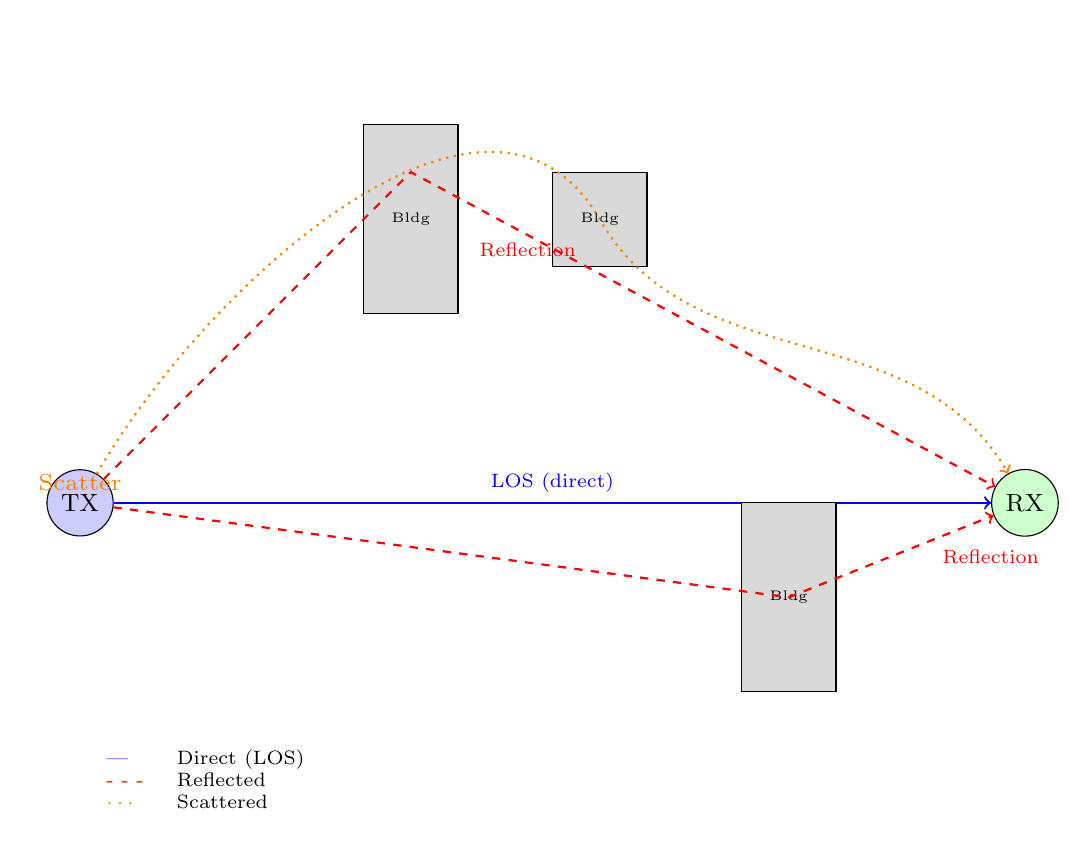
\begin{tikzpicture}[scale=1.2]
% Transmitter
\node[draw, circle, minimum size=0.8cm, fill=blue!20] (tx) at (0,0) {\small TX};

% Receiver
\node[draw, circle, minimum size=0.8cm, fill=green!20] (rx) at (10,0) {\small RX};

% Direct path (LOS)
\draw[->, thick, blue] (tx) -- (rx) node[midway, above] {\scriptsize LOS (direct)};

% Buildings
\draw[fill=gray!30] (3,2) rectangle (4,4) node[midway] {\tiny Bldg};
\draw[fill=gray!30] (7,-2) rectangle (8,0) node[midway] {\tiny Bldg};
\draw[fill=gray!30] (5,2.5) rectangle (6,3.5) node[midway] {\tiny Bldg};

% Reflected paths
\draw[->, thick, red, dashed] (tx) -- (3.5,3.5) -- (rx) node[pos=0.3, above left] {\scriptsize Reflection};
\draw[->, thick, red, dashed] (tx) -- (7.5,-1) -- (rx) node[pos=0.7, below right] {\scriptsize Reflection};

% Scattered path
\draw[->, thick, orange, dotted] (tx) to[out=60, in=120] (5.5,3) to[out=-60, in=120] (rx) node[pos=0.5, above] {\scriptsize Scatter};

% Legend
\node[anchor=north west, font=\scriptsize] at (0,-2.5) {
\begin{tabular}{ll}
\textcolor{blue}{---} & Direct (LOS) \\
\textcolor{red}{- - -} & Reflected \\
\textcolor{orange}{$\cdots$} & Scattered
\end{tabular}
};
\end{tikzpicture}
\end{center}

\subsection{Reflection}

Electromagnetic waves bounce off surfaces including ground (two-ray model), buildings (urban canyons), water bodies (maritime communications), and the ionosphere (HF skywave propagation).

The \textbf{Fresnel reflection coefficient} for perpendicular polarization is:
\begin{equation}
\Gamma_\perp = \frac{\cos\theta_i - \sqrt{\epsilon_r - \sin^2\theta_i}}{\cos\theta_i + \sqrt{\epsilon_r - \sin^2\theta_i}}
\end{equation}
where:
\begin{itemize}
\item $\Gamma_\perp$ = reflection coefficient (magnitude)
\item $\theta_i$ = angle of incidence
\item $\epsilon_r$ = relative permittivity of surface material
\end{itemize}

\textbf{Example:} Concrete wall at 2.4~GHz has $\epsilon_r \approx 6$, yielding $|\Gamma| \approx 0.3$--0.5 (corresponding to 3--6~dB loss per bounce).

\subsection{Diffraction}

Diffraction enables waves to \textbf{bend around obstacles} such as building edges, hills/terrain, and vegetation. This Fresnel diffraction phenomenon extends coverage into shadowed (NLOS) regions.

The \textbf{knife-edge diffraction loss} is:
\begin{equation}
L_d \approx 6 + 20\log_{10}\left(\sqrt{(v-0.1)^2 + 1} + v - 0.1\right) \quad \text{(dB)}
\end{equation}
where:
\begin{itemize}
\item $L_d$ = diffraction loss (dB)
\item $v$ = Fresnel-Kirchhoff diffraction parameter (dimensionless)
\end{itemize}

The Fresnel parameter is given by:
\begin{equation}
v = h\sqrt{\frac{2(d_1 + d_2)}{\lambda d_1 d_2}}
\end{equation}
where:
\begin{itemize}
\item $h$ = height of obstacle above line-of-sight path (m)
\item $d_1, d_2$ = distances from transmitter and receiver to obstacle (m)
\item $\lambda$ = wavelength (m)
\end{itemize}

\subsection{Scattering}

Scattering occurs when waves interact with rough surfaces or objects comparable to or smaller than the wavelength: rough terrain (vegetation, rocks), lamp posts, street signs, and rain/fog droplets (at high frequencies).

For \textbf{Rayleigh scattering} (object size $\ll \lambda$), the scattered power follows:
\begin{equation}
P_{\text{scattered}} \propto \frac{1}{\lambda^4}
\end{equation}
where:
\begin{itemize}
\item $P_{\text{scattered}}$ = scattered power
\item $\lambda$ = wavelength
\end{itemize}

This strong wavelength dependence explains why blue light (shorter $\lambda$) scatters more than red light in the atmosphere, creating blue skies. In RF systems, higher frequencies experience more scattering loss.

\section{Time-Domain Effects}

\subsection{Delay Spread}

Multipath components arrive at the receiver with different delays, creating \textbf{delay spread}. The RMS delay spread characterizes this temporal dispersion:

\begin{equation}
\tau_{\text{rms}} = \sqrt{\frac{\sum_{i=1}^N P_i (\tau_i - \bar{\tau})^2}{\sum_{i=1}^N P_i}}
\end{equation}
where:
\begin{itemize}
\item $\tau_{\text{rms}}$ = RMS delay spread (seconds)
\item $P_i$ = power of path $i$
\item $\tau_i$ = delay of path $i$
\item $\bar{\tau}$ = mean delay = $\frac{\sum P_i \tau_i}{\sum P_i}$
\item $N$ = number of resolvable paths
\end{itemize}

The following diagram illustrates delay spread in the time domain:

\begin{center}
\begin{tikzpicture}[scale=1.0]
% Axes
\draw[->] (0,0) -- (10,0) node[right] {Time (relative delay $\tau$)};
\draw[->] (0,0) -- (0,4) node[above] {Power};

% Direct path (earliest arrival)
\draw[->, thick, blue] (1,0) -- (1,3.5) node[above] {\scriptsize LOS};
\fill[blue] (1,3.5) circle (2pt);

% Reflected paths (delayed arrivals)
\draw[->, thick, red] (2.5,0) -- (2.5,2.0);
\fill[red] (2.5,2.0) circle (2pt);

\draw[->, thick, red] (4,0) -- (4,1.5);
\fill[red] (4,1.5) circle (2pt);

\draw[->, thick, red] (5.5,0) -- (5.5,0.8);
\fill[red] (5.5,0.8) circle (2pt);

\draw[->, thick, orange] (7,0) -- (7,0.5);
\fill[orange] (7,0.5) circle (2pt);

% Mean delay
\draw[dashed, gray] (3.2,0) -- (3.2,3.8) node[above, font=\scriptsize] {$\bar{\tau}$};

% RMS spread indication
\draw[<->, thick, gray] (2.2,-0.5) -- (5.2,-0.5) node[midway, below, font=\scriptsize] {$\approx \tau_{\text{rms}}$};

% Labels
\node[font=\scriptsize] at (5,-1.5) {Multipath arrivals spread over time};
\end{tikzpicture}
\end{center}

\textbf{Typical $\tau_{\text{rms}}$ values:}
\begin{itemize}
\item \textbf{Rural/suburban}: 0.1--1~$\mu$s
\item \textbf{Urban}: 1--5~$\mu$s
\item \textbf{Indoor}: 10--100~ns
\end{itemize}

\subsection{Coherence Bandwidth}

The \textbf{coherence bandwidth} $B_c$ defines the frequency range over which the channel response is approximately flat (constant amplitude and linear phase):

\begin{equation}
B_c \approx \frac{1}{5\tau_{\text{rms}}}
\end{equation}
where:
\begin{itemize}
\item $B_c$ = coherence bandwidth (Hz)
\item $\tau_{\text{rms}}$ = RMS delay spread (seconds)
\end{itemize}

\begin{warningbox}
If signal bandwidth $B > B_c$, the channel exhibits \textbf{frequency-selective fading}---different frequency components fade independently, causing \textbf{intersymbol interference (ISI)}. Equalization or OFDM is required.
\end{warningbox}

\textbf{Example:} Urban environment with $\tau_{\text{rms}} = 1~\mu$s:
\begin{equation}
B_c \approx \frac{1}{5 \times 10^{-6}} = 200~\text{kHz}
\end{equation}

\textbf{Classification:}
\begin{itemize}
\item \textbf{Narrowband signal} ($B < 200$~kHz): Flat fading (all frequencies fade together)
\item \textbf{Wideband signal} ($B > 200$~kHz): Frequency-selective fading (ISI present)
\end{itemize}

\subsection{Intersymbol Interference (ISI)}

Delayed multipath components overlap with subsequent symbols, causing \textbf{intersymbol interference}. The condition for significant ISI is:
\begin{equation}
\tau_{\text{rms}} > T_s
\end{equation}
where:
\begin{itemize}
\item $T_s$ = symbol period (seconds)
\item $\tau_{\text{rms}}$ = RMS delay spread (seconds)
\end{itemize}

\textbf{Example:} 1~Mbps data rate ($T_s = 1~\mu$s) in urban channel ($\tau_{\text{rms}} = 3~\mu$s):

The condition $\tau_{\text{rms}} > T_s$ is satisfied ($3 > 1$), meaning \textbf{ISI is severe}---up to 3 symbols overlap simultaneously!

\textbf{Mitigation:} Channel equalization (see Chapter~\ref{ch:equalization}) or OFDM (see Chapter~\ref{ch:ofdm}) is required to combat ISI.

\section{Frequency-Domain Effects}

\subsection{Doppler Shift}

Relative motion between transmitter and receiver causes a \textbf{Doppler frequency shift}:
\begin{equation}
f_d = \frac{v}{\lambda} \cos(\theta) = \frac{v \cdot f_c}{c} \cos(\theta)
\end{equation}
where:
\begin{itemize}
\item $f_d$ = Doppler shift (Hz)
\item $v$ = relative velocity (m/s)
\item $\lambda$ = wavelength (m)
\item $\theta$ = angle between velocity vector and signal direction
\item $f_c$ = carrier frequency (Hz)
\item $c$ = speed of light ($3 \times 10^8$~m/s)
\end{itemize}

\textbf{Example:} Vehicle at 100~km/h (27.8~m/s), 2~GHz signal, direct approach ($\theta = 0°$):
\begin{equation}
f_d = \frac{27.8 \times 2 \times 10^9}{3 \times 10^8} \cos(0°) = 185~\text{Hz}
\end{equation}

\subsection{Doppler Spread}

In multipath environments, different paths have different Doppler shifts due to varying angles of arrival. The \textbf{Doppler spread} is:
\begin{equation}
B_d = 2f_{d,\text{max}} = \frac{2v}{\lambda} = \frac{2v \cdot f_c}{c}
\end{equation}
where:
\begin{itemize}
\item $B_d$ = Doppler spread (Hz)
\item $f_{d,\text{max}}$ = maximum Doppler shift (Hz)
\end{itemize}

The \textbf{coherence time} characterizes how long the channel remains approximately constant:
\begin{equation}
T_c \approx \frac{0.423}{B_d}
\end{equation}
where:
\begin{itemize}
\item $T_c$ = coherence time (seconds)
\item $B_d$ = Doppler spread (Hz)
\end{itemize}

\textbf{Example:} 100~km/h at 2~GHz:
\begin{equation}
B_d = 2 \times 185 = 370~\text{Hz}
\end{equation}
\begin{equation}
T_c = \frac{0.423}{370} = 1.14~\text{ms}
\end{equation}

\textbf{Implication:} Channel changes every $\sim$1~ms. This is \textbf{fast fading} for low data rates but \textbf{slow fading} for high-speed systems where many symbols transmit within $T_c$.

\subsection{Fading Classifications}\label{fading-classifications}

\subsubsection{Flat vs
Frequency-Selective}\label{flat-vs-frequency-selective}

{\def\LTcaptype{} % do not increment counter
\begin{longtable}[]{@{}
  >{\raggedright\arraybackslash}p{(\linewidth - 6\tabcolsep) * \real{0.1622}}
  >{\raggedright\arraybackslash}p{(\linewidth - 6\tabcolsep) * \real{0.2973}}
  >{\raggedright\arraybackslash}p{(\linewidth - 6\tabcolsep) * \real{0.2162}}
  >{\raggedright\arraybackslash}p{(\linewidth - 6\tabcolsep) * \real{0.3243}}@{}}
\toprule\noalign{}
\begin{minipage}[b]{\linewidth}\raggedright
Type
\end{minipage} & \begin{minipage}[b]{\linewidth}\raggedright
Condition
\end{minipage} & \begin{minipage}[b]{\linewidth}\raggedright
Effect
\end{minipage} & \begin{minipage}[b]{\linewidth}\raggedright
Mitigation
\end{minipage} \\
\midrule\noalign{}
\endhead
\bottomrule\noalign{}
\endlastfoot
\textbf{Flat} & \(B \ll B_c\) & All frequencies fade together &
Diversity, FEC \\
\textbf{Frequency-selective} & \(B \gg B_c\) & Different frequencies
fade independently & Equalization, OFDM \\
\end{longtable}
}

\begin{center}\rule{0.5\linewidth}{0.5pt}\end{center}

\subsubsection{Fast vs Slow Fading}\label{fast-vs-slow-fading}

{\def\LTcaptype{} % do not increment counter
\begin{longtable}[]{@{}
  >{\raggedright\arraybackslash}p{(\linewidth - 6\tabcolsep) * \real{0.1622}}
  >{\raggedright\arraybackslash}p{(\linewidth - 6\tabcolsep) * \real{0.2973}}
  >{\raggedright\arraybackslash}p{(\linewidth - 6\tabcolsep) * \real{0.2162}}
  >{\raggedright\arraybackslash}p{(\linewidth - 6\tabcolsep) * \real{0.3243}}@{}}
\toprule\noalign{}
\begin{minipage}[b]{\linewidth}\raggedright
Type
\end{minipage} & \begin{minipage}[b]{\linewidth}\raggedright
Condition
\end{minipage} & \begin{minipage}[b]{\linewidth}\raggedright
Effect
\end{minipage} & \begin{minipage}[b]{\linewidth}\raggedright
Mitigation
\end{minipage} \\
\midrule\noalign{}
\endhead
\bottomrule\noalign{}
\endlastfoot
\textbf{Slow} & \(T_c \gg T_s\) & Channel constant over many symbols &
Interleaving, FEC \\
\textbf{Fast} & \(T_c \ll T_s\) & Channel changes within symbol &
Pilot-aided estimation \\
\end{longtable}
}

\begin{center}\rule{0.5\linewidth}{0.5pt}\end{center}

\section{Rayleigh Fading}

\textbf{Rayleigh fading} occurs when there is \textbf{no dominant line-of-sight (LOS) path} and the received signal consists of many scattered components with random phases.

\begin{keyconcept}
When numerous multipath components with random phases combine, the Central Limit Theorem predicts that the in-phase and quadrature components are Gaussian distributed. The signal \textbf{envelope} then follows a Rayleigh distribution.
\end{keyconcept}

\subsection{Mathematical Description}

The \textbf{probability density function (PDF)} of the Rayleigh envelope is:
\begin{equation}
p_R(r) = \frac{r}{\sigma^2} \exp\left(-\frac{r^2}{2\sigma^2}\right), \quad r \geq 0
\end{equation}
where:
\begin{itemize}
\item $r$ = signal envelope amplitude
\item $\sigma^2$ = average power of in-phase or quadrature component
\item Total average power: $\Omega = 2\sigma^2$
\end{itemize}

The \textbf{mean} and \textbf{variance} are:
\begin{equation}
\bar{r} = \sigma\sqrt{\frac{\pi}{2}} = \sqrt{\frac{\pi \Omega}{4}}
\end{equation}
\begin{equation}
\text{Var}(r) = \sigma^2\left(2 - \frac{\pi}{2}\right) = \frac{\Omega}{2}\left(2 - \frac{\pi}{2}\right)
\end{equation}

\subsection{Cumulative Distribution Function}

The \textbf{CDF} gives the probability that the signal envelope falls below a threshold $R$:
\begin{equation}
F_R(R) = P(r < R) = 1 - \exp\left(-\frac{R^2}{2\sigma^2}\right)
\end{equation}
where:
\begin{itemize}
\item $F_R(R)$ = probability of signal below threshold $R$
\item $R$ = threshold level
\end{itemize}

\textbf{Example:} Probability signal drops 10~dB below average (i.e., $R = 0.316\bar{r}$):
\begin{equation}
P(r < 0.316\bar{r}) = 1 - \exp\left(-\frac{(0.316\bar{r})^2}{2\sigma^2}\right) = 1 - \exp(-0.05) \approx 5\%
\end{equation}

This shows Rayleigh fading causes frequent deep fades---the signal drops more than 10~dB about 5\% of the time.

\subsection{PDF Comparison: Rayleigh vs Rician}

\begin{center}
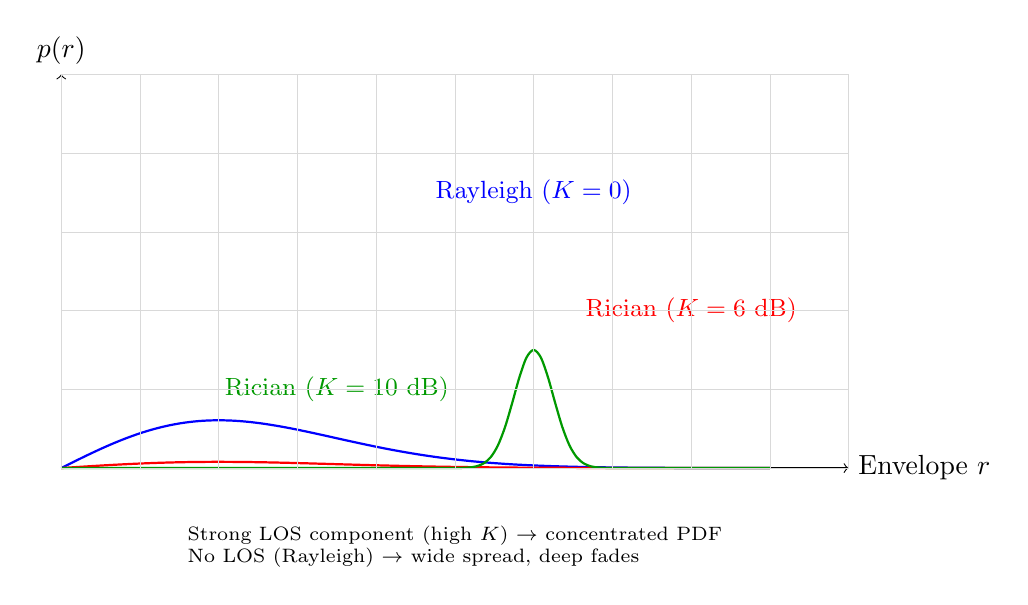
\begin{tikzpicture}[scale=1.0]
% Axes
\draw[->] (0,0) -- (10,0) node[right] {Envelope $r$};
\draw[->] (0,0) -- (0,5) node[above] {$p(r)$};

% Rayleigh PDF (K=0)
\draw[thick, blue, domain=0:9, samples=100, smooth] plot (\x, {(\x/2)*exp(-(\x*\x)/8)});
\node[blue, font=\small] at (6,3.5) {Rayleigh ($K=0$)};

% Rician K=6 dB (K=4)
\draw[thick, red, domain=0:9, samples=100, smooth] plot (\x, {0.8*(\x/2)*exp(-(\x*\x + 16)/8)*1.2});
\node[red, font=\small] at (8,2) {Rician ($K=6$~dB)};

% Rician K=10 dB (K=10) - more concentrated
\draw[thick, green!60!black, domain=0:9, samples=100, smooth] plot (\x, {(\x > 5 && \x < 7) ? 1.5*exp(-8*(\x-6)*(\x-6)) : 0});
\node[green!60!black, font=\small] at (3.5,1) {Rician ($K=10$~dB)};

% Grid
\draw[gray!30, very thin] (0,0) grid[step=1] (10,5);

% Annotations
\node[font=\scriptsize, align=left] at (5,-1) {
Strong LOS component (high $K$) $\rightarrow$ concentrated PDF\\
No LOS (Rayleigh) $\rightarrow$ wide spread, deep fades
};
\end{tikzpicture}
\end{center}

\subsection{Impact on BER}

Rayleigh fading \textbf{severely degrades} bit error rate performance. For \textbf{coherent BPSK} in Rayleigh fading:
\begin{equation}
\text{BER}_{\text{Rayleigh}} = \frac{1}{2}\left(1 - \sqrt{\frac{\bar{\gamma}}{1 + \bar{\gamma}}}\right)
\end{equation}
where:
\begin{itemize}
\item $\bar{\gamma} = \frac{E_b}{N_0}$ = average SNR per bit
\end{itemize}

Compare this to AWGN performance:
\begin{equation}
\text{BER}_{\text{AWGN}} = Q\left(\sqrt{2\bar{\gamma}}\right)
\end{equation}

\textbf{Comparison at $\bar{\gamma} = 10$~dB:}
\begin{itemize}
\item \textbf{AWGN channel}: BER = $3.9 \times 10^{-6}$
\item \textbf{Rayleigh fading}: BER = $0.005$ (\textbf{1000× worse!})
\end{itemize}

\begin{calloutbox}{Physical Explanation}
Deep fades push the instantaneous SNR into the noise floor, causing \textbf{error bursts}. Even though fades are brief, they dominate the average BER. This is why diversity and coding are essential for fading channels.
\end{calloutbox}

\subsection{Typical Rayleigh Environments}

Rayleigh fading is characteristic of:
\begin{itemize}
\item \textbf{Dense urban areas}: No LOS, many reflections from buildings (urban canyons)
\item \textbf{Indoor environments}: Office buildings, corridors, shopping malls
\item \textbf{Suburban/rural NLOS}: Heavy vegetation, obstructions blocking direct path
\item \textbf{Mobile-to-mobile communications}: Both terminals moving, no stable LOS
\end{itemize}

\section{Rician Fading}

\textbf{Rician fading} occurs when there is a \textbf{dominant line-of-sight (LOS) path} plus additional scattered components. The Rician distribution generalizes the Rayleigh distribution by adding a deterministic LOS component.

\subsection{Mathematical Description}

The \textbf{Rician PDF} is:
\begin{equation}
p_{\text{Ric}}(r) = \frac{r}{\sigma^2} \exp\left(-\frac{r^2 + A^2}{2\sigma^2}\right) I_0\left(\frac{Ar}{\sigma^2}\right), \quad r \geq 0
\end{equation}
where:
\begin{itemize}
\item $r$ = envelope amplitude
\item $A$ = amplitude of LOS component
\item $\sigma^2$ = average power of scattered components (per quadrature)
\item $I_0(\cdot)$ = modified Bessel function of the first kind, order zero
\end{itemize}

The \textbf{Rician K-factor} characterizes the ratio of LOS to scattered power:
\begin{equation}
K = \frac{A^2}{2\sigma^2} = \frac{\text{LOS power}}{\text{Scattered power}}
\end{equation}

In decibels:
\begin{equation}
K_{\text{dB}} = 10\log_{10}(K)
\end{equation}

\begin{keyconcept}
When $K = 0$ (no LOS), the Rician distribution \textbf{reduces to Rayleigh}. As $K \to \infty$ (pure LOS), the channel approaches AWGN. The K-factor thus interpolates between Rayleigh and AWGN behavior.
\end{keyconcept}

\subsection{Interpretation of K-factor}

\begin{center}
\begin{tabular}{lll}
\toprule
\textbf{K (dB)} & \textbf{Environment} & \textbf{Fading Severity} \\
\midrule
$-\infty$ ($K=0$) & No LOS (pure Rayleigh) & \textbf{Severe} (deep fades) \\
0~dB ($K=1$) & Equal LOS/scatter & Moderate \\
6~dB ($K=4$) & Strong LOS & Mild \\
10~dB ($K=10$) & Dominant LOS & Negligible fading \\
$+\infty$ & Pure LOS (AWGN-like) & None \\
\bottomrule
\end{tabular}
\end{center}

As K-factor increases, the channel becomes more deterministic (less fading). System designers measure K-factor to predict link reliability.

\subsection{Impact on BER}

Rician fading is \textbf{less severe than Rayleigh} due to the stabilizing influence of the LOS component. For coherent BPSK in Rician fading, the BER is (approximate):
\begin{equation}
\text{BER}_{\text{Rician}} \approx Q\left(\sqrt{\frac{2K\bar{\gamma}}{K+1}}\right) \exp\left(-\frac{K\bar{\gamma}}{K+1}\right) \left[1 + \text{correction terms}\right]
\end{equation}
where $K$ is the linear K-factor and $\bar{\gamma} = E_b/N_0$.

\textbf{Performance comparison at $\bar{\gamma} = 10$~dB:}
\begin{itemize}
\item \textbf{AWGN}: BER = $3.9 \times 10^{-6}$
\item \textbf{Rician} $K=6$~dB: BER $\approx 10^{-5}$ (10× worse than AWGN)
\item \textbf{Rayleigh} ($K=0$): BER = $0.005$ (1000× worse than AWGN)
\end{itemize}

The strong LOS component in Rician channels significantly improves reliability compared to pure Rayleigh fading.

\subsection{Typical Rician Environments}

Rician fading is characteristic of:
\begin{itemize}
\item \textbf{Suburban areas}: Partial LOS with moderate scattering
\item \textbf{Elevated antennas}: Rooftop base stations with clear path to users
\item \textbf{Satellite-to-handheld}: Weak LOS component plus ground reflections (K typically 5--10~dB)
\item \textbf{Indoor near windows}: LOS to outdoor base station plus indoor multipath
\item \textbf{Rural areas}: Clear LOS with minimal scattering (high K-factor)
\end{itemize}

\section{Fade Statistics}

\subsection{Fade Margin}

Link budgets must include \textbf{fade margin} to maintain target availability in the presence of fading. The minimum received power is:
\begin{equation}
P_r(\text{min}) = P_r(\text{average}) - M_{\text{fade}}
\end{equation}
where:
\begin{itemize}
\item $P_r(\text{average})$ = average received power (dBm)
\item $M_{\text{fade}}$ = fade margin (dB)
\item $P_r(\text{min})$ = minimum acceptable received power (dBm)
\end{itemize}

\textbf{Required fade margins for target availability:}

\textbf{Rayleigh fading:}
\begin{itemize}
\item 90\% availability: $M_{\text{fade}} \approx 10$~dB
\item 99\% availability: $M_{\text{fade}} \approx 20$~dB
\item 99.9\% availability: $M_{\text{fade}} \approx 30$~dB
\end{itemize}

\textbf{Rician fading} ($K = 6$~dB):
\begin{itemize}
\item 90\% availability: $M_{\text{fade}} \approx 5$~dB
\item 99\% availability: $M_{\text{fade}} \approx 10$~dB
\item 99.9\% availability: $M_{\text{fade}} \approx 15$~dB
\end{itemize}

\subsection{Level Crossing Rate (LCR)}

The \textbf{level crossing rate} quantifies how often the signal envelope crosses a threshold $R$ (in crossings per second):
\begin{equation}
N_R = \sqrt{2\pi} \cdot f_d \cdot \rho \cdot \exp(-\rho^2)
\end{equation}
where:
\begin{itemize}
\item $N_R$ = level crossing rate (crossings/sec)
\item $f_d$ = maximum Doppler frequency (Hz)
\item $\rho = R/R_{\text{rms}}$ = normalized threshold level
\item $R_{\text{rms}}$ = RMS signal level
\end{itemize}

\textbf{Example:} Mobile at 100~km/h, 2~GHz ($f_d = 185$~Hz), threshold = average power ($\rho = 1$):
\begin{equation}
N_R = \sqrt{2\pi} \times 185 \times 1 \times \exp(-1) \approx 85~\text{fades/sec}
\end{equation}

The signal crosses the average power level about 85 times per second---very rapid fading!

\subsection{Average Fade Duration}

The \textbf{average fade duration} is the mean time the signal stays below threshold $R$:
\begin{equation}
\bar{t} = \frac{\exp(\rho^2) - 1}{\rho f_d \sqrt{2\pi}}
\end{equation}
where $\bar{t}$ is in seconds.

\textbf{Example:} Same scenario ($f_d = 185$~Hz, $\rho = 1$):
\begin{equation}
\bar{t} = \frac{e - 1}{1 \times 185 \times \sqrt{2\pi}} \approx 3.7~\text{ms}
\end{equation}

\textbf{Implication:} Fast fading (85 fades/sec) with short fade durations ($\sim$4~ms) means \textbf{interleaving is effective}---error bursts can be spread across multiple codewords for FEC to correct.

\section{Worked Example: Urban LTE Link Analysis}

\begin{calloutbox}{Complete Calculation}
\textbf{Scenario:} Design an LTE uplink for urban environment.

\textbf{Given parameters:}
\begin{itemize}
\item Frequency: $f_c = 1.8$~GHz (LTE Band 3)
\item Mobile velocity: $v = 50$~km/h = 13.9~m/s
\item RMS delay spread: $\tau_{\text{rms}} = 2~\mu$s (typical urban)
\item Channel model: Rayleigh fading (NLOS)
\item Target: 1~Mbps QPSK, 99\% link availability
\end{itemize}

\textbf{Step 1: Calculate coherence bandwidth}
\begin{equation}
B_c = \frac{1}{5\tau_{\text{rms}}} = \frac{1}{5 \times 2 \times 10^{-6}} = 100~\text{kHz}
\end{equation}

LTE resource block (RB) bandwidth is 180~kHz $> B_c$, so the channel is \textbf{frequency-selective}. OFDM is essential.

\textbf{Step 2: Calculate Doppler spread}

Wavelength: $\lambda = c/f_c = 3 \times 10^8 / 1.8 \times 10^9 = 0.167$~m

Maximum Doppler:
\begin{equation}
f_{d,\text{max}} = \frac{v}{\lambda} = \frac{13.9}{0.167} = 83.3~\text{Hz}
\end{equation}

Doppler spread:
\begin{equation}
B_d = 2 f_{d,\text{max}} = 167~\text{Hz}
\end{equation}

\textbf{Step 3: Calculate coherence time}
\begin{equation}
T_c = \frac{0.423}{B_d} = \frac{0.423}{167} = 2.53~\text{ms}
\end{equation}

LTE subframe duration is 1~ms $< T_c$, so channel is \textbf{slow fading}. Channel estimation per subframe is sufficient.

\textbf{Step 4: Required fade margin (99\% availability)}

For Rayleigh fading, 99\% availability requires approximately \textbf{20~dB fade margin}.

If average received power is $P_{\text{avg}} = -80$~dBm, minimum power must be:
\begin{equation}
P_{\text{min}} = -80 - 20 = -100~\text{dBm}
\end{equation}

The receiver sensitivity must be better than $-100$~dBm to maintain 99\% availability.

\textbf{Step 5: BER in Rayleigh fading}

For QPSK in Rayleigh fading with average $E_b/N_0 = 15$~dB:
\begin{equation}
\text{BER} \approx \frac{1}{2}\left(1 - \sqrt{\frac{\bar{\gamma}}{1 + \bar{\gamma}}}\right) \approx 0.001
\end{equation}

This is \textbf{100× worse} than AWGN performance at the same average SNR.

\textbf{Conclusion:}
\begin{itemize}
\item OFDM required (frequency-selective fading)
\item Channel changes slowly enough for tracking (slow fading)
\item 20~dB fade margin needed
\item Strong FEC (e.g., Turbo codes) essential to combat fading
\end{itemize}
\end{calloutbox}

\section{Performance Analysis}

\subsection{BER Performance Comparison}

The following diagram illustrates BER performance for BPSK across different channel models:

\begin{center}
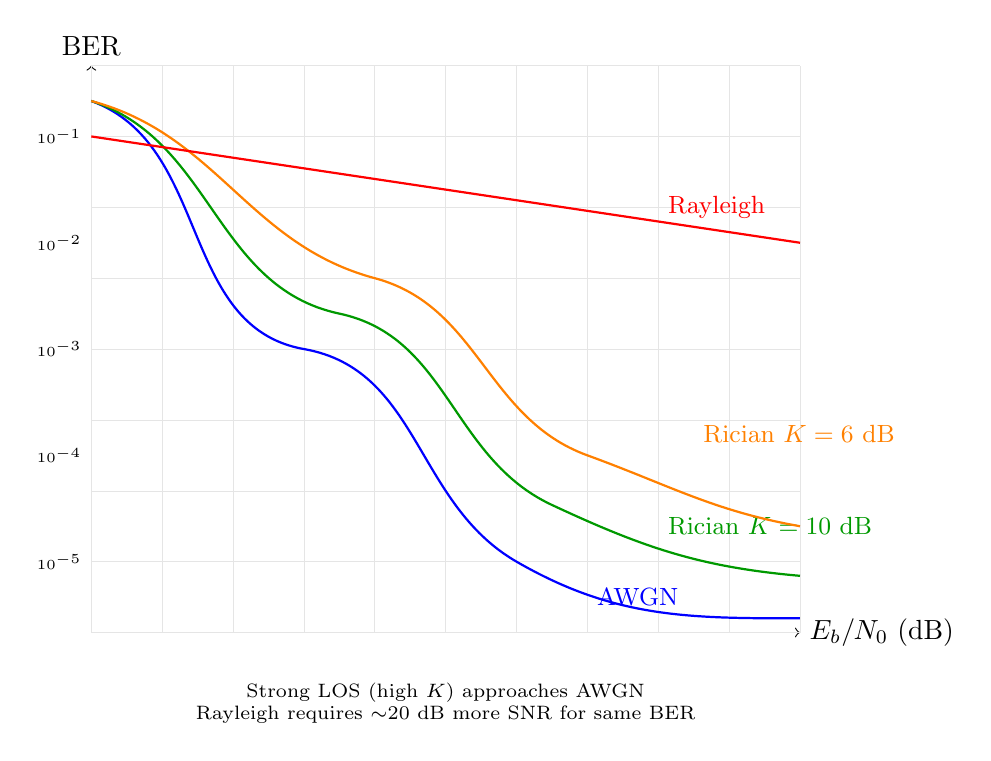
\begin{tikzpicture}[scale=0.9]
% Axes
\draw[->] (0,0) -- (10,0) node[right] {$E_b/N_0$ (dB)};
\draw[->] (0,0) -- (0,8) node[above] {BER};

% Log scale labels (indicative)
\node[left, font=\tiny] at (0,7) {$10^{-1}$};
\node[left, font=\tiny] at (0,5.5) {$10^{-2}$};
\node[left, font=\tiny] at (0,4) {$10^{-3}$};
\node[left, font=\tiny] at (0,2.5) {$10^{-4}$};
\node[left, font=\tiny] at (0,1) {$10^{-5}$};

% Grid
\draw[gray!20, very thin] (0,0) grid[step=1] (10,8);

% AWGN curve (steep, best performance)
\draw[thick, blue] (0,7.5) to[out=-20, in=170] (3,4) to[out=-10, in=150] (6,1) to[out=-30, in=180] (10,0.2);
\node[blue, font=\small, anchor=west] at (7,0.5) {AWGN};

% Rician K=10 dB (close to AWGN)
\draw[thick, green!60!black] (0,7.5) to[out=-18, in=168] (3.5,4.5) to[out=-12, in=155] (6.5,1.8) to[out=-25, in=175] (10,0.8);
\node[green!60!black, font=\small, anchor=west] at (8,1.5) {Rician $K=10$ dB};

% Rician K=6 dB
\draw[thick, orange] (0,7.5) to[out=-15, in=165] (4,5) to[out=-15, in=160] (7,2.5) to[out=-20, in=170] (10,1.5);
\node[orange, font=\small, anchor=west] at (8.5,2.8) {Rician $K=6$ dB};

% Rayleigh (worst, nearly flat)
\draw[thick, red] (0,7) -- (10,5.5);
\node[red, font=\small, anchor=west] at (8,6) {Rayleigh};

% Annotations
\node[font=\scriptsize, align=center] at (5,-1) {
Strong LOS (high $K$) approaches AWGN\\
Rayleigh requires $\sim$20 dB more SNR for same BER
};
\end{tikzpicture}
\end{center}

At a target BER of $10^{-3}$, Rayleigh fading requires approximately \textbf{20~dB more} $E_b/N_0$ than AWGN---a massive penalty that demands mitigation.

\section{Mitigation Techniques}

\subsection{1. Diversity}

Diversity exploits the fact that independent fading signals are unlikely to simultaneously experience deep fades.

\textbf{Spatial diversity} (antenna diversity): Use multiple antennas separated by $d > \lambda/2$. Selection combining provides $\sim$10~dB improvement with 2 antennas.

\textbf{Frequency diversity}: Transmit same data on multiple frequencies separated by $> B_c$. Application: frequency-hopping spread spectrum (FHSS).

\textbf{Time diversity}: Transmit same data at different times separated by $> T_c$. Implementation: interleaving combined with FEC spreads coded bits over time.

\subsection{2. Equalization}

Equalization compensates for frequency-selective fading (ISI). The zero-forcing equalizer inverts the channel:
\begin{equation}
H_{\text{eq}}(f) = \frac{1}{H_{\text{channel}}(f)}
\end{equation}

\textbf{Problem:} Noise amplification at deep channel nulls.

\textbf{Decision-feedback equalization (DFE)} uses past decisions to cancel ISI without noise amplification.

\textbf{Adaptive equalization} tracks time-varying channels using LMS or RLS algorithms with periodic pilot symbols for training.

\subsection{3. OFDM}

Orthogonal Frequency Division Multiplexing (OFDM) divides wideband signals into many narrowband subcarriers. Each subcarrier bandwidth $< B_c$ experiences flat fading, enabling simple single-tap equalization per subcarrier. See Chapter~\ref{ch:ofdm} for details.

\subsection{4. Spread Spectrum}

Spreading the signal over wide bandwidth provides frequency diversity---different frequency components fade independently. See Chapter~\ref{ch:spread} for DSSS and FHSS techniques.

\subsection{5. Forward Error Correction}

FEC with interleaving protects against error bursts. Interleaving spreads coded bits across time/frequency so that fade-induced burst errors appear as isolated errors to the decoder, which are easier to correct. Turbo codes, LDPC codes, and polar codes provide robust performance. See Chapters~\ref{ch:fec} and~\ref{ch:ldpc}.

\section{Applications}

Multipath fading is the dominant channel impairment in numerous wireless systems:

\subsection{Practical Examples}\label{practical-examples}

\subsubsection{Example 1: Urban Cellular (900
MHz)}\label{example-1-urban-cellular-900-mhz}

\textbf{Environment}: Dense urban, NLOS

\textbf{Parameters}: - Delay spread: \(\tau_{\text{rms}} = 3\ \mu\)s -
Doppler: \(f_d = 50\) Hz (30 km/h) - Fading: Rayleigh

\textbf{Coherence bandwidth}:

\[
B_c = \frac{1}{5 \times 3 \times 10^{-6}} = 67\ \text{kHz}
\]

\textbf{Implication}: GSM channel (200 kHz) experiences
frequency-selective fading \$\textbackslash rightarrow\$ Equalizer
needed

\textbf{Coherence time}:

\[
T_c = \frac{0.423}{100} = 4.23\ \text{ms}
\]

\textbf{Implication}: Channel constant over \textasciitilde18 GSM
symbols (0.577 ms/symbol) \$\textbackslash rightarrow\$ Slow fading

\begin{center}\rule{0.5\linewidth}{0.5pt}\end{center}

\subsubsection{Example 2: Suburban LTE (2.6
GHz)}\label{example-2-suburban-lte-2.6-ghz}

\textbf{Environment}: Suburban, partial LOS

\textbf{Parameters}: - Delay spread: \(\tau_{\text{rms}} = 0.5\ \mu\)s -
Doppler: \(f_d = 240\) Hz (100 km/h) - Fading: Rician K=5 dB

\textbf{Coherence bandwidth}:

\[
B_c = \frac{1}{5 \times 0.5 \times 10^{-6}} = 400\ \text{kHz}
\]

\textbf{Implication}: LTE RB (180 kHz) \textless{} \(B_c\)
\$\textbackslash rightarrow\$ Mostly flat fading per RB

\textbf{Coherence time}:

\[
T_c = \frac{0.423}{480} = 0.88\ \text{ms}
\]

\textbf{Implication}: Channel changes over \textasciitilde12 OFDM
symbols (71 \$\textbackslash mu\$s/symbol) \$\textbackslash rightarrow\$
Moderate fading, pilot-aided tracking

\begin{center}\rule{0.5\linewidth}{0.5pt}\end{center}

\subsection{Summary Table}\label{summary-table}

{\def\LTcaptype{} % do not increment counter
\begin{longtable}[]{@{}
  >{\raggedright\arraybackslash}p{(\linewidth - 6\tabcolsep) * \real{0.2500}}
  >{\raggedright\arraybackslash}p{(\linewidth - 6\tabcolsep) * \real{0.2273}}
  >{\raggedright\arraybackslash}p{(\linewidth - 6\tabcolsep) * \real{0.3864}}
  >{\raggedright\arraybackslash}p{(\linewidth - 6\tabcolsep) * \real{0.1364}}@{}}
\toprule\noalign{}
\begin{minipage}[b]{\linewidth}\raggedright
Parameter
\end{minipage} & \begin{minipage}[b]{\linewidth}\raggedright
Rayleigh
\end{minipage} & \begin{minipage}[b]{\linewidth}\raggedright
Rician (K=6 dB)
\end{minipage} & \begin{minipage}[b]{\linewidth}\raggedright
AWGN
\end{minipage} \\
\midrule\noalign{}
\endhead
\bottomrule\noalign{}
\endlastfoot
\textbf{LOS component} & None & Dominant & Pure LOS \\
\textbf{Fade depth (10\% time)} & -10 dB & -5 dB & 0 dB \\
\textbf{BER penalty @ 10 dB SNR} & 1000\$\textbackslash times\$ &
10\$\textbackslash times\$ & 1\$\textbackslash times\$ (baseline) \\
\textbf{Mitigation} & Diversity, FEC & Moderate FEC & Minimal FEC \\
\textbf{Typical environment} & Dense urban, indoor & Suburban, elevated
& Free space, satellite \\
\end{longtable}
}

\begin{center}\rule{0.5\linewidth}{0.5pt}\end{center}

\subsection{Related Topics}\label{related-topics}

\begin{itemize}
\tightlist
\item
  \textbf{{[}{[}Propagation-Modes-(Ground-Wave,-Sky-Wave,-Line-of-Sight){]}{]}}:
  LOS vs NLOS propagation
\item
  \textbf{{[}{[}Atmospheric-Effects-(Ionospheric,-Tropospheric){]}{]}}:
  Clear-air effects (different from multipath)
\item
  \textbf{{[}{[}Signal-to-Noise-Ratio-(SNR){]}{]}}: Fading reduces
  instantaneous SNR
\item
  \textbf{{[}{[}Bit-Error-Rate-(BER){]}{]}}: Fading degrades BER
  significantly
\item
  \textbf{{[}{[}QPSK-Modulation{]}{]}} /
  \textbf{{[}{[}LDPC-Codes{]}{]}}: Require fade mitigation
\item
  \textbf{{[}{[}OFDM-\&-Multicarrier-Modulation{]}{]}}: Combats
  frequency-selective fading
\item
  \textbf{{[}{[}Spread-Spectrum-(DSSS-FHSS){]}{]}}: Provides frequency
  diversity
\end{itemize}

\begin{center}\rule{0.5\linewidth}{0.5pt}\end{center}

\textbf{Key takeaway}: \textbf{Multipath fading is the dominant
impairment} in mobile/urban wireless. Rayleigh fading (no LOS) is
severe, Rician fading (with LOS) is moderate. Mitigation requires
diversity, equalization, OFDM, and robust FEC. Understanding \(B_c\) and
\(T_c\) is critical for system design.

\begin{center}\rule{0.5\linewidth}{0.5pt}\end{center}

\emph{This wiki is part of the {[}{[}Home\textbar Chimera Project{]}{]}
documentation.}
